
\subsection{Постановка проблемы}
Инвариантная спиновая ось частицы, учавствующей в бетатронном движении, колеблется вокруг своего референсного значения.~\cite[стр.~11]{Shatunov} По этой причине, амплитуда решения уравнения Т-БМТ для вертикальной компоненты спин-вектора:
\begin{align}
s_y &= \sqrt{\bkt{\frac{\w_y\w_z}{\w}}^2 + \bkt{\frac{\w_x}{\w}}^2}\cdot\sin\bkt{\w\cdot t + \phi}\notag\\
&= \sqrt{\bkt{\bar n_y\bar n_z}^2 + \bar n_x^2} \cdot \sin\bkt{2\pi\cdot\nu_s\cdot n_{turn} + \phi},\label{eq:sy_varying_amplitude}
\end{align}
превращается в изменяющуюся во времени функцию. Если вариация оси стабильного спина (а также спин-тюна частицы) имеет достаточно большую амплитуду, использование гармонической функции с постоянными параметрами в качестве модели для фитирования сигнала повлечёт за собой систематическую ошибку спецификации модели. Ошибки данного типа отражаются на валидности оценок параметров модели, то есть на оценке частоты, и потому требуют анализа.

Вариация спин-тюна $\nu_s$ особенно проблематична в этом отношении, т.к. она напрямую влияет на фазу сигнала; однако, эта проблема может быть решена введением в ускорительную структуру секступольных полей, как описано в разделе~\ref{sec:sextupole_spin_dec_solution}. В связи с этим, в настоящем разделе мы сфокусируемся на рассмотрении вариации $\bar n$.

\subsection{Численное моделирование}
Симуляция проводилась следующим образом: частица, смещённая с референсной орбиты в вертикальном направлении
на 0.3 мм, многократно инжектируется в неидеальную структуру с замороженным спином~\cite{Senichev:Lattices},
использующую секступоли для подавления декогеренции, вызванной бетатронными колебаниями
в вертикальной плоскости (см. раздел~\ref{sec:sextupole_spin_dec_solution}).
Неидеальности структуры симулируются наклонами E+B элементов.
Введённые таким образом неидеальности не ведут к возмущению референсной орбиты (то есть,
референсная орбита --- равно как и орбита бетатрон-осциллирующей частицы --- одинакова для всех инжекций.)

На каждой инжекции, углы наклонов E+B элементов генерируются случайным образом из
нормального распределения $\alpha\sim N(\mu_i, 3\cdot 10^{-4})$ градусов, $i\in\{1,\dots,11\}$, где
$\mu_i$ изменяется в диапазоне $[-1.5\cdot10^{-4}, +2.5\cdot10^{-4}]$ градусов. Ненулевые ожидания $\mu_i$
симулируют введение в систему Кооп-Колеса.~\cite{Koop:SpinWheel} Величины $\mu_i$ и $\sigma_{\alpha}$
выбраны с целью детализации эффекта. При больших значениях, труднее различимы эффекты влияния вариации
$\nu_s$ и $\bar n$.

Ещё одним аспектом симуляции, требующим упоминания, является то, что частица инжектируется на энергии 270 МэВ, в то время как условие замороженности спина выполняется строго при 270.0092 МэВ. Из-за этого, ось стабильного спина $\nbar$ смотрит в основном в вертикальном направлении (отклоняясь от него не более чем на \ang{51} при больших скоростях поворота Кооп-Колеса); её радиальная компонента (определяющая амплитуду колебаний вертикальной компоненты спин-вектора) относительно мала, и потому ещё более чувствительна к вариации, вызванной бетатронным движением в вертикальной плоскости.

Трэкинг спина выполнялся с помощью кода COSY Infinity~\cite{COSYINF:Website}, на протяжении $1.2\cdot10^6$
оборотов; каждые 800 оборотов $\nu_s$ и $\bar n$ вычисляются (процедурой
TSS~\cite[стр.~41]{COSYINF:Manual:BeamPhys}) в точке фазового пространства, занимаемой частицей на данный момент,
что даёт нам серию $(\nu_s(n), \bar n(n))$, $n$ --- номер оборота частицы в ускорителе.
Соответствующие компоненты спин-вектора $(s_x^{trk}(n), s_y^{trk}(n), s_z^{trk}(n))$,
вычисленные трэкером (процедура TR~\cite[стр.~41]{COSYINF:Manual:BeamPhys}), составляют вторую серию данных,
используемых в анализе.

\subsection{Анализ}
Используя данные первой серии, мы сгенерировали ожидаемую $s_y^{gen}(t)$ ``генераторную'' серию,
в соответствии с уравнением~\eqref{eq:sy_varying_amplitude}, а также ``идеальную'' серию $s_y^{idl}$, в которой
мы положили постоянные значения $\nu_s = \avg{\nu_s(t)}$ и $\bar n =\avg{\bar n(t)}$. 

Наша гипотеза состоит в том, что бетатронное движение частицы
должно ввести несоответствие между синусоидальной моделью
\begin{equation}
  f(t) = a\cdot\sin(\w\cdot t + \delta),\label{eq:fit_model}
\end{equation}
и данными трекера, путём вариации оси прецессии спина $\bar n$, а значит амплитуды
фитируемого сигнала. ``Идеальная'' серия служит базой сравнительного анализа,
так как она идеально соответствует модели; ``генераторная'' серия учитывает вариацию $\bar n$,
всё ещё оставаясь в пределах модели. ``Трекерная'' серия --- наиболее близкое приближение
к реальным измерительным данным.

Для сравнения серий между собой, мы
\begin{enumerate*}[\itshape a\upshape)]
\item вычислили и проанализировали невязки $\epsilon_1(t) = s_y^{gen}(t) -
  s_y^{idl}(t)$ и $\epsilon_2(t) = s_y^{trk}(t) - s_y^{idl}(t)$;
\item профитировали модель~\eqref{eq:fit_model} к трём сериям данных, и
  сравнили качество фита;
\item вычислили стандартные отклонения компонент $\bar n$ при каждом
  значении скорости Спин-Колеса.
\end{enumerate*}

\begin{figure}[h]
	\centering
	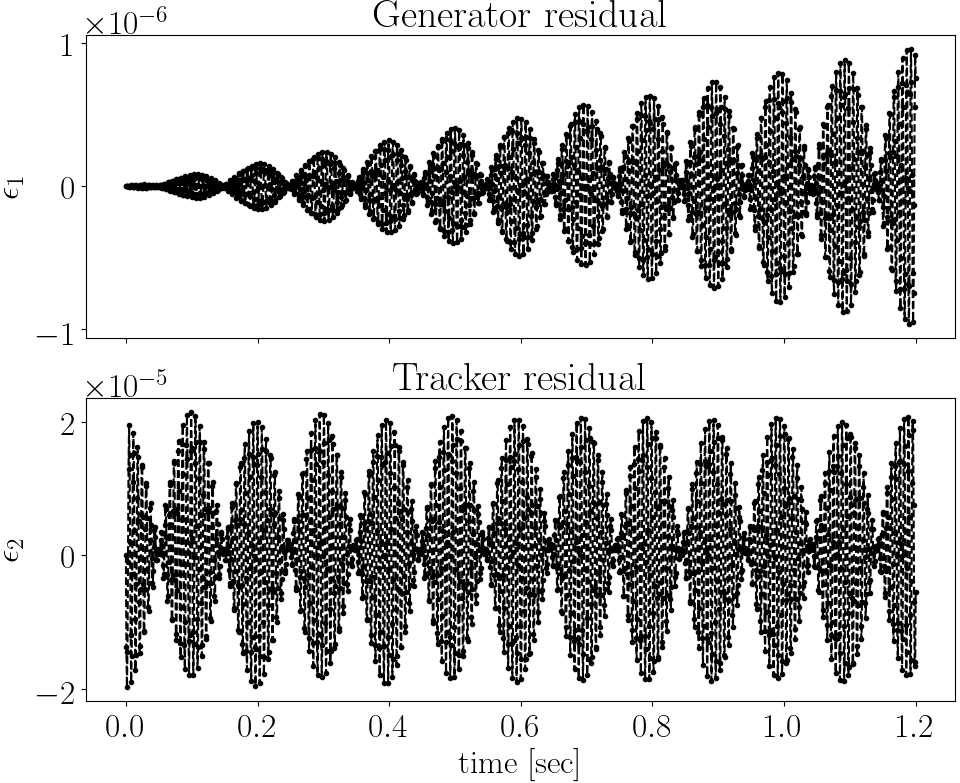
\includegraphics[height=.35\paperheight]{images/smp_sim/residual_vs_time(both)}
	\caption{Сравнительные невязки как функции времени.
		Верхняя панель: невязка $\epsilon_1$; нижняя панель: невязка $\epsilon_2$\label{fig:residuals}}
\end{figure}

\begin{figure}[h]
  \centering
	\subbottom[Компонент $\bar n$\label{fig:sd:nbar}]{%
    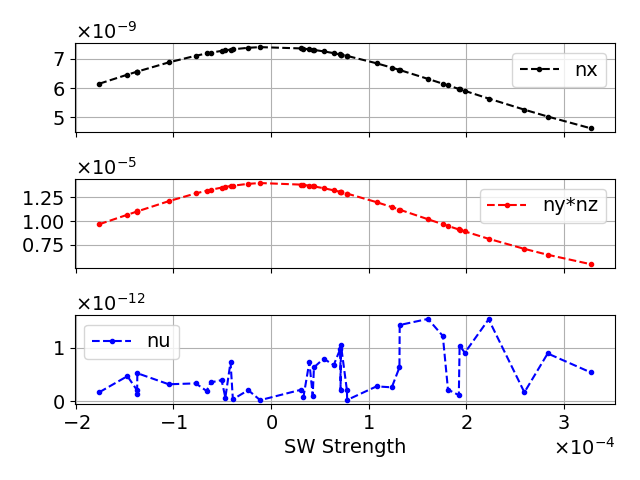
\includegraphics[height=.35\paperheight]{images/smp_sim/NBAR_variation_sd_vs_SW}}
	\subbottom[Сравнительных невязок.
	Верхняя панель: невязка $\epsilon_1$; нижняя панель: невязка $\epsilon_2$\label{fig:sd:res}]{%
    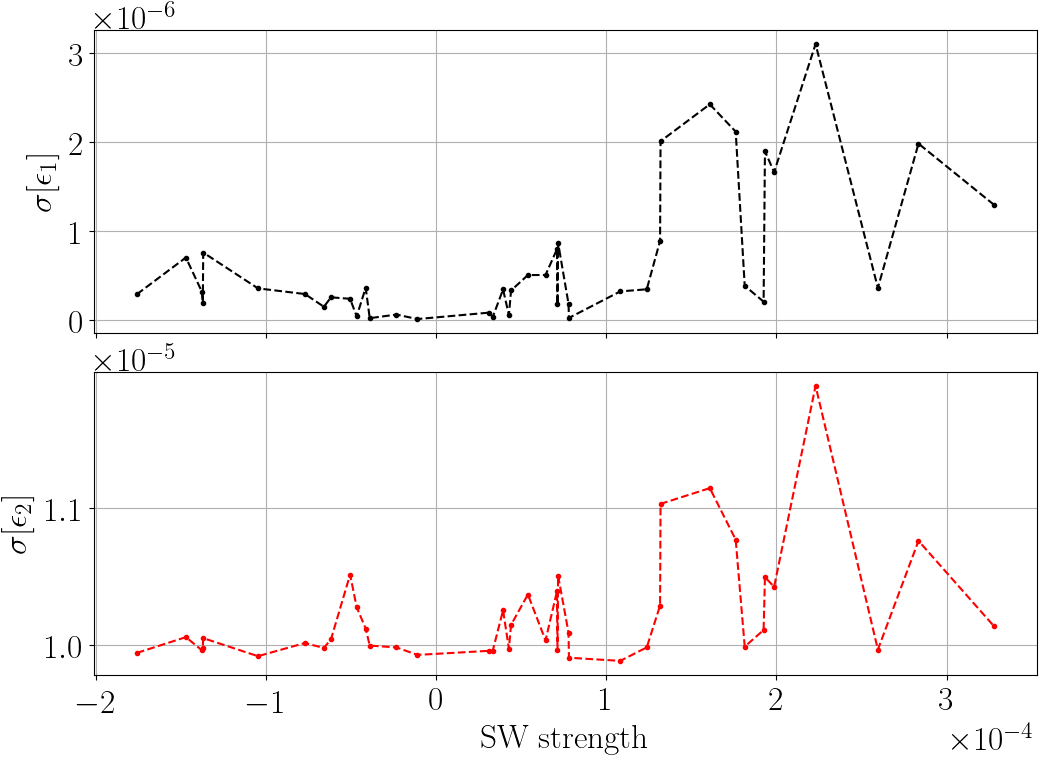
\includegraphics[height=.35\paperheight]{images/smp_sim/residual_SD_vs_SW(both)}}
  \caption{Стандартные отклонения против относительной скорости Спин-Колеса\label{fig:sd}}
\end{figure}

\begin{table}[h]\centering
	\caption{Оценки параметров модели (медленный SW)\label{tbl:param_estimates}}
	\begin{tabular}{r|rllr}
		\toprule
		Серия & Пар. & Величина & Ст.Ошибка & AIC \\
		\midrule
		\multirow{3}{*}{$s_y^{idl}$}
		& $\hat f$ & 4.220359687911 & $6.9\cdot10^{-11}$ & \multirow{3}{*}{-62093} \\
		& $\hat a$ & 0.12514597851 & $4\cdot10^{-11}$ & \\
		& $\hat\delta$ & $-1.50\cdot10^{-8}$ & $4\cdot 10^{-10}$ &\\
		\hline
		\multirow{3}{*}{$s_y^{gen}$}
		& $\hat f$ & 4.2203596911 & $1.9\cdot 10^{-9}$ & \multirow{3}{*}{-52142} \\
		& $\hat a$ & 0.125145979 & $1\cdot 10^{-9}$ & \\
		& $\hat\delta$ & $-1.6\cdot 10^{-8}$ & $1.2\cdot 10^{-8}$ &\\
		\hline
		\multirow{3}{*}{$s_y^{trk}$}
		& $\hat f$ & 4.2203603 & $1.3\cdot 10^{-6}$ & \multirow{3}{*}{-34567} \\
		& $\hat a$ & 0.12514597 & $3.7\cdot10^{-7}$ & \\
		& $\hat\delta$ & $-4\cdot10^{-6}$ & $6\cdot 10^{-6}$ &\\
		\bottomrule
	\end{tabular}
\end{table}


На Рисунке~\ref{fig:residuals} мы наблюдаем, что ``генераторная'' серия почти идентична
``идеальной'' серии, при $\epsilon_1 \le 1\cdot10^{-6}$ (даже если её частота немного отличается) в течении длительности цикла,
в то время как ``трекерная'' серия отклоняется от неё на уровне
$\epsilon_2 \le 2\cdot 10^{-5}$.  Это различие между $\epsilon_1$ и $\epsilon_2$ наблюдается
систематически для всех величин скорости Спин-Колеса (см. Рисунок~\ref{fig:sd:res}), и пока что не имеет объяснения.

На Рисунке~\ref{fig:sd:res} мы наблюдаем, что стандартные отклонения обеих невязок показывают такую же зависимость от скорости колеса, как и $\nu_s$ (Рисунок~\ref{fig:sd:nbar}, нижняя панель), но не как стандартное отклонение компонент $\bar n$.
Это свидетельствует о том, что вариация частоты даёт значительно больший вклад в несоответствие между
моделью~\eqref{eq:fit_model} и трекерными данными, чем предполагаемая вариация амплитуды, вызванная изменением ориентации $\bar n$.

Таблица~\ref{tbl:param_estimates} характеризует качество фита модели по отношению к данным,
в случае самого медленного Кооп-Колеса.
Видно, что попарные разницы между оценками параметров серий не являются статистически-значимыми. Хотя вариация вектора угловой скорости спин-прецессии ухудшила качество фита модели, она не ввела никакого статистически-значимого систематического смещения в оценки.


\subsection{Выводы}
Вопрос влияния бетатронного движения на ЭДМ статистику в FD-методологии следует рассматривать
ввиду трёх обстоятельств:
\begin{enumerate}
\item Осцилляции амплитуды сигнала очень малы. Они происходят на уровне не более $10^{-4}$ (при
  $\alpha\sim N(0, 3\cdot 10^{-2})$ градусов), тогда как ожидаемая неточность измерений поляризации находится
  на уровне процентов. Это значит суперпозиция систематической ошибки и случайной ошибки измерения
  не будет проявлять статистически-значимую систематичность.
\item Коэффициент корреляции между оценками амплитуды и частоты не значителен. Колебания амплитуды
  влияюи на оценку $\hat a$ в первую очередь; их эффект на оценку $\hat\w$ опосредован, и описывается
  коэффициентом корреляции. Поскольку он меньше 10\%, даже если колебания окажутся достаточными, чтобы повлиять
  на оценку амплитуды, их эффект на оценку частоты будет уменьшен по крайней мере в 10 раз.
\item Этот систематический эффект контролируется. И этот фактор является основным достоинством методологий
  частотной области. Вводя в систему внешнее Спин-Колесо, колебания $\bar n$ могут быть непрерывно минимизированы
  до необходимого уровня, без каких-либо модификаций паттерна эксперимента.
\end{enumerate}
